\documentclass[a4paper,12pt]{report}

% Page layout
\usepackage[left=2.5cm,right=2.5cm,top=2.5cm,bottom=2.5cm]{geometry}

% Font and text
\usepackage[afrikaans,english]{babel}
\usepackage{microtype}
\usepackage{setspace}
\usepackage{lmodern}
\usepackage{siunitx}
\newcommand{\myemph}[1]{{\sffamily\bfseries#1}}
\sloppy
\onehalfspacing

% Headings
\usepackage[raggedright,sf,bf]{titlesec}
\usepackage[margin=\the\parindent,small,bf,sf]{caption}
\titlelabel{\thetitle.\ }
\titleformat{\chapter}[display]{\huge\bfseries\sffamily}{\chaptertitlename\ \thechapter}{15pt}{\Huge \raggedright}
\titlespacing*{\chapter}{0pt}{0pt}{40pt}  % remove spacing before chapter headings
\makeatletter
\let\originall@chapter\l@chapter
\def\l@chapter#1#2{\originall@chapter{{\sffamily #1}}{#2}}
\makeatother

%% Alternative headings using small-caps (comment out the top section)
%\usepackage[raggedright,bf]{titlesec}
%\usepackage[margin=\the\parindent,small,bf]{caption}
%\titlelabel{\thetitle.\ }
%\titleformat{\chapter}[display]{\huge\scshape}{\chaptertitlename\ \thechapter}{15pt}{\Huge \raggedright}
%\titlespacing*{\chapter}{0pt}{0pt}{40pt}  % remove spacing before chapter headings

% Table of contents
\let \savenumberline \numberline
\def \numberline#1{\savenumberline{#1.}}

% Figures
\usepackage{graphicx}
\usepackage{pdfpages}
\usepackage{subcaption}
\setlength{\abovecaptionskip}{7.5pt}  % spacing above and below captions
\newcommand*{\WaterMark}[2][0.2\paperwidth]{\AddToShipoutPicture*{\AtTextCenter{\parbox[c]{0pt}{\makebox[0pt][c]{\includegraphics[width=#1]{#2}}}}}}

% Mathematics
\usepackage[cmex10]{amsmath}
\usepackage{amssymb}
\usepackage{cancel}
\DeclareMathOperator*{\argmax}{arg\,max}
\newcommand{\T}{^\top}
\newcommand{\tr}{\textrm{tr}}
\renewcommand{\vec}[1]{\boldsymbol{\mathbf{#1}}}
\newcommand{\defeq}{\triangleq}

% Tables
\usepackage{booktabs}
\usepackage{tabularx}
\usepackage{multirow}
\newcommand{\mytable}{
    \centering
    \small
    \renewcommand{\arraystretch}{1.2}
    }
\renewcommand{\tabularxcolumn}[1]{m{#1}}
\newcolumntype{C}{>{\centering\arraybackslash}X}
\newcolumntype{L}{>{\raggedright\arraybackslash}X}
% added self
\usepackage{makecell}  % Include makecell for multiline cells

% Header and footer
\usepackage{fancyhdr}
\pagestyle{fancy}
\fancyhf{}
\renewcommand{\sectionmark}[1]{\markright{\normalsize \thesection.\ #1}}
\fancyhead[C]{\nouppercase{\textit{\rightmark}}}
\fancyhead[RO]{\thepage}
 \fancyhead[LE]{\thepage}  % double-sided printing
\fancyfoot{}
\setlength\headheight{14.5pt}
\renewcommand{\headrulewidth}{0pt}
\fancypagestyle{plain}{\fancyhead{}
                       \renewcommand{\headrulewidth}{0pt}
                       \fancyfoot[C]{\thepage}}

% Pseudo-code
\usepackage{algorithm}  % should go before \usepackage{hyperref}

% Table of contents and hyperlinks
\usepackage{hyperref}
\hypersetup{colorlinks=true,linktoc=all,citecolor=black,linkcolor=black}
\usepackage[nottoc]{tocbibind}

% Pseudo-code
\usepackage{algpseudocode}  % should go after \usepackage{hyperref}
\renewcommand{\thealgorithm}{\arabic{chapter}.\arabic{algorithm}} 
\captionsetup[algorithm]{labelfont={bf,sf},font=small,labelsep=colon}

% Bibliography
\usepackage{cite}  % automatically reorder inline citations
\bibliographystyle{IEEEtran}

% Fix titlesec issue
\usepackage{etoolbox}
\makeatletter
\patchcmd{\ttlh@hang}{\parindent\z@}{\parindent\z@\leavevmode}{}{}
\patchcmd{\ttlh@hang}{\noindent}{}{}{}
\makeatother


\begin{document}

% Front matter
% \graphicspath{{frontmatter/fig/}}
% \pagenumbering{Alph}

% \begin{titlepage}
% 	\begin{center}
		
% 		
\includegraphics[width=10cm]{USlogo-top}
		
% 		\vfill
		
% 		{\sffamily \bfseries \huge Synthesis and Evaluation of an Image-Based GNSS-Redundancy System for UAV Navigation \par}
% %		{\scshape \huge A Critical Analysis of Design Flaws in the Death Star \par}
		
% 		\vfill
		
% 		{\large {\Large Sameer Shaboodien} \\ 25002783 \par}
		
% 		\vfill
		
% 		\vfill
		
% 		{Report submitted in partial fulfilment of the requirements of the module \\
% 			Project (E) 448 for the degree Baccalaureus in Engineering in the Department of
% 			Electrical and Electronic Engineering at Stellenbosch University. \par}
		
% 		\vfill
		
% 		{\large {Supervisor}: Dr R.\ P.\ Theart} %\\
% 		% Department of Electrical and Electronic Engineering \par}
		
% 		\vfill
		
% 		{\Large October 2024}
% 	\end{center}
% \end{titlepage}



\graphicspath{{frontmatter/fig/}}
\pagenumbering{Alph}

\begin{titlepage}
	\begin{tikzpicture}[remember picture, overlay]
        \node [opacity=1.0, anchor=center] at (current page.center) 
        {
\includegraphics[width=1.1\paperwidth]{stb-thesis-frntp.pdf}};
    \end{tikzpicture}
	\begin{center}
		
%		\includegraphics[width=10cm]{SU_corporate_horizontal_with_slogan_RGB}
        % \includegraphics[width=3.75cm]{SU_corporate_vertical_without_slogan_RGB-crop}
				
		\vfill
		\vfill
        \vfill
		
		{\bfseries \huge Synthesis and Evaluation of an Image-Based GNSS-Redundancy System for UAV Navigation \par}
%		{\scshape \huge A Critical Analysis of Design Flaws in the Death Star \par}
		
		\vfill
		
        {\large by \\[5pt]}
		{\Large {\Large Sameer Shaboodien \\ 25002783} \par}
		
		\vfill
		
		\vfill
		
		% Skripsie
		{\large Report presented in partial fulfilment of the requirements of the module \\ Project (E) 448 for the degree Baccalaureus in Engineering (Electrical and Electronic) in the Faculty of Engineering at Stellenbosch University. \par}
		
		% Masters (Research)
		% {\large Thesis presented in fulfilment of the requirements for the degree of \\ Master of Engineering (Electronic) in the Faculty of Engineering at Stellenbosch University. \par}
		
		% Masters (Structured)
		% {\large Research assignment presented in partial fulfilment of the requirements for the degree of Master of Engineering (Electronic) \\ in the Faculty of Engineering at Stellenbosch University. \par}
		
		% PhD
		% {\large Dissertation presented for the degree of Doctor of Philosophy (Electronic Engineering) in the Faculty of Engineering at Stellenbosch University. \par}
		
		\vfill
		
		{\large {Supervisor}: Prof. RP Theart}\par
        % {\large {Co-supervisor}: Prof. Q.\ G.\ Jinn}
		
		\vfill
		
		{\large 01 November 2024}
               \vfill
	\end{center}
\end{titlepage}
%\graphicspath{{frontmatter/fig/}}
\pagenumbering{Alph}

\begin{titlepage}
	\begin{center}
		
		%
\includegraphics[width=10cm]{USlogo-top}
		
		\WaterMark{UScrest-WM}
		
		~\vspace{4.5em}
		
		{\sffamily \bfseries \huge Synthesis and Evaluation of an Image-Based Redundancy System for Enhanced UAV Navigation \par}
%		{\scshape \huge A Critical Analysis of Design Flaws in the Death Star \par}		
		
		\vspace{7em}
		
		{\large {\Large  Sameer Shaboodien} \\ 25002783 \par}
		
		\vspace{8em}
		
		{\large Thesis presented in partial fulfilment of the requirements for the degree of \\ Master of Engineering (Electronic) in the Faculty of Engineering at Stellenbosch University. \par}
		
		\vfill
		
		{\large {Supervisor}: Dr R.\ P.\ Theart\\
		Department of Electrical and Electronic Engineering \par}
		
		%\vfill
		\vspace{10em}
		
		{\Large October 2024}
	\end{center}
\end{titlepage}

\pagenumbering{roman}
\chapter*{Acknowledgements}
% \addcontentsline{toc}{chapter}{Acknowledgements}
\makeatletter\@mkboth{}{Acknowledgements}\makeatother

I would like to thank my dog, Muffin. I also would like to thank the inventor of the incubator; without him/her, I would not be here. Finally, I would like to thank Dr Herman Kamper for this amazing report template.
%\chapter*{Declaration}
\newpage
\thispagestyle{plain}
\addcontentsline{toc}{chapter}{Declaration}
\makeatletter\@mkboth{}{Declaration}\makeatother

\centerline{
\includegraphics[width=8cm]{USlogo-top}}
\vspace*{-10pt}

\section*{\centering Plagiaatverklaring / \textit{Plagiarism Declaration}}

\vspace*{5pt}

\begin{enumerate}
    \item Plagiaat is die oorneem en gebruik van die idees, materiaal en ander intellektuele eiendom van ander persone asof dit jou eie werk is.\\
    \textit{Plagiarism is the use of ideas, material and other intellectual property of another's work
        and to present is as my own.}
    
    \item Ek erken dat die pleeg van plagiaat 'n strafbare oortreding is aangesien dit 'n vorm van diefstal is.\\
    \textit{I agree that plagiarism is a punishable offence because it constitutes theft.}
    
    \item Ek verstaan ook dat direkte vertalings plagiaat is. \\
    \textit{I also understand that direct translations are plagiarism.}
    
    \item Dienooreenkomstig is alle aanhalings en bydraes vanuit enige bron (ingesluit die internet) volledig verwys (erken). Ek erken dat die woordelikse aanhaal van teks sonder aanhalingstekens (selfs al word die bron volledig erken) plagiaat is. \\
    \textit{Accordingly all quotations and contributions from any source whatsoever (including the internet) have been cited fully. I understand that the reproduction of text without quotation marks (even when the source is cited) is plagiarism}
    
    \item Ek verklaar dat die werk in hierdie skryfstuk vervat, behalwe waar anders aangedui, my eie oorspronklike werk is en dat ek dit nie vantevore in die geheel of gedeeltelik ingehandig het vir bepunting in hierdie module/werkstuk of 'n ander module/werkstuk~nie. \\
    \textit{I declare that the work contained in this assignment, except where otherwise stated, is my original work and that I have not previously (in its entirety or in part) submitted it for grading in this module/assignment or another module/assignment.}
\end{enumerate}

\vfill

\noindent \begin{tabularx}{1.0\linewidth}{|L|L|}
    \hline
    \vspace{1cm} {Studentenommer / \textit{25002783}} & \vspace{1cm} {Handtekening / \textit{SamS}} \\
    \hline
    \vspace{1cm} {Voorletters en van / \textit{S Shaboodien}} & \vspace{1cm} {Datum / \textit{27/10/24}} \\
    \hline
\end{tabularx}

\vspace{15pt}

% The old declaration

%I, the undersigned, hereby declare that the work contained in this report is my own original work unless otherwise stated.
%
%% Afrikaans:
%% Hiermee verklaar ek, die ondergetekende, dat die werk in hierdie verslag vervat my eie oorspronklike werk is, tensy anders vermeld.
%
%\vspace{2.5cm}
%
%\begin{table}[h]
%\begin{tabular}{@{}p{2.5cm}p{5cm}}
%    Signature: & \dotfill \\
%    & \multicolumn{1}{c}{Obi-Wan Kenobi} \\
%    ~\vspace{1cm} \\
%    Date: & \dotfill \\
%\end{tabular}
%\end{table}
%
%\vfill
%
%\begin{center}
%    Copyright \textcopyright\ 2099 Stellenbosch University \\
%    All rights reserved
%\end{center}


\chapter*{Abstract}
\addcontentsline{toc}{chapter}{Abstract}
\makeatletter\@mkboth{}{Abstract}\makeatother

% \subsubsection*{English}



Unmanned Aerial Vehicles (UAVs) rely on the Global Positioning System (GPS) for precise navigation, but vulnerabilities such as jamming and spoofing can jeopardize mission success. This project developed an image-based GPS localization system to enable reliable UAV navigation in GPS-denied environments. The system optimizes the localization pipeline by integrating advanced feature extraction, matching, and planar transformation techniques, achieving radial localization errors below 10\% of the UAV's displacement from a reference image. Designed for real-time operation, the system responds within two seconds after GPS signal loss, allowing pilots to maintain effective control. Comprehensive testing across diverse environments demonstrated the system's high accuracy, robustness, and generalizability without requiring environment-specific tuning. The system excelled in low-light and low-overlap conditions, ensuring dependable navigation data delivery in various scenarios. This image-based localization provides a practical and reliable alternative to GPS, enhancing UAV operational safety and effectiveness in both military and civilian applications. With further enhancements, the system is poised for real-world deployment, promising safer and more reliable UAV missions.




\selectlanguage{afrikaans}

% \subsubsection*{Afrikaans}



% Onbemande Lugvaartuie (UAV's) is afhanklik van die Globale Positieseringsstelsel (GPS) vir presiese navigasie, maar kwesbaarhede soos storings en spogging kan missie-sukses in gevaar stel. Hierdie projek het 'n beeld-gebaseerde GPS-lokaliseringsstelsel ontwikkel om betroubare UAV-navigasie in GPS-ontkende omgewings moontlik te maak. Die stelsel optimaliseer die lokalisasie-pyplyn deur gevorderde kenmerkuittrekking, ooreenstemming en planêre transformasie tegnieke te integreer, en bereik radiale lokalisasie-foute onder 10\% van die UAV se verskuiwing vanaf 'n verwysingsbeeld. Ontwerp vir regstreekse operasie, reageer die stelsel binne twee sekondes na GPS-siggewigsverlies, wat vlieërs in staat stel om effektiewe beheer te behou. Omvattende toetsing oor diverse omgewings het die stelsel se hoë akkuraatheid, robuustheid en generaliseerbaarheid getoon sonder om omgewings-spesifieke afstelling nodig te hê. Die stelsel het uitnemend gepresteer in lae-lig en lae-ooreenkoms toestande, wat betroubare navigasiedata lewer in verskeie scenario's. Hierdie beeld-gebaseerde lokalisasie bied 'n praktiese en betroubare alternatief vir GPS, wat UAV-operasionele veiligheid en doeltreffendheid in beide militêre en siviele toepassings verbeter. Met verdere verbeterings is die stelsel gereed vir werklike implementering, wat veiliger en meer betroubare UAV-missies belowe.





\selectlanguage{english}
\tableofcontents
\listoffigures
\listoftables
\chapter*{Nomenclature\markboth{}{Nomenclature}}
\addcontentsline{toc}{chapter}{Nomenclature}

% \vspace*{-3mm}
\subsubsection*{Variables and Functions}

\begingroup
\renewcommand{\arraystretch}{1.2}
\renewcommand{\tabularxcolumn}[1]{p{#1}}
\begin{tabularx}{\textwidth}{@{}p{2.5cm}L}
    $RMSE$ & Root Mean Square Error, representing the average magnitude of errors. In this study, the usage of this metric specifically, and frequently, uses this term to refer to the radial error in GPS estimate, in metres, averaged across the dataset. \\
    $d_{\text{radial}}$ & Radial error distance, measuring the distance between estimated and true positions in meters.\\
    $x$, $y$ & Coordinates of a point in an image or on the ground plane.\\
    $\theta$ & Rotation angle between consecutive images in degrees or radians, used for orientation alignment.\\
    $T$ & Transformation matrix representing the planar transformation between images.\\
    $H$ & Homography matrix, specifically mapping points from one image plane to another.\\
    $GPS$ & Global Positioning System, providing geolocation and time information for navigation.\\
    $GNSS$ & Global Navigation Satellite System, a generic term for satellite-based navigation systems.\\

    $MAE$ & Mean Absolute Error, measuring the average localization error without directionality.\\
    $MI$ & Mutual Information, measuring the similarity or overlap between images, often used in image matching.\\
\end{tabularx}
\endgroup

\newpage
\subsubsection*{Key Terms and Concepts}

\begingroup
\renewcommand{\arraystretch}{1.2}
\begin{tabularx}{\textwidth}{@{}p{2.5cm}L}

    \textbf{Features} & 
    Unique keypoints in an image along with their descriptors, used for identifying and uniquely matching points across different images for localization. \\
    
    \textbf{Affine Transformation} & 
    A planar transformation that preserves points, straight lines, and planes, including translation, scaling, rotation, and shearing. \\


    \textbf{Descriptors} & 
    Numerical values describing the characteristics of keypoints in an image, allowing for effective matching between different images. \\

    \textbf{Feature Detectors (or Extractors)} & 
    Processes for identifying distinct features in an image, which are invariant to changes in scale, rotation, and illumination. \\



    \textbf{Global Matching} & 
    Process of finding similarities and determining pose between entire images, considering full-image context rather than isolated keypoints. \\

    \textbf{GPS (Global Positioning System)} & 
    A satellite navigation system providing geolocation and time information. Vulnerable to jamming and spoofing, posing reliability issues for UAV navigation. \\

    \textbf{Homography} & 
    A planar transformation mapping points from one image plane to another in 2D space. Used in image processing to describe transformations like rotation, translation, scaling, and shearing. \\

    \textbf{Homography Estimation} & 
    The process of calculating the homography matrix that defines the transformation between two images for alignment and reliable localization. \\

    \textbf{Keypoints} & 
    Specific points in an image used to identify features. Typically areas of strong contrast or distinct patterns, enabling reliable matching across different images. \\

    \textbf{Local Matching} & 
    Matching keypoints between images by comparing descriptors, focusing on individual feature descriptors to establish precise localization. \\

    \textbf{Mutual Information} & 
    A metric quantifying the information shared between two images, aiding in assessing the quality of feature matching and overlap similarity. \\

    \textbf{Planar Transforms} & 
    General transformations applied to a plane in 2D space, such as affine transformations, homography, scaling, and shearing, which are crucial for image alignment. \\

    \textbf{Scaling} & 
    A transformation that changes the size of an image or its features without altering its shape, normalizing feature sizes across different images. \\

    \textbf{Shearing} & 
    A type of affine transformation that slants the shape of an object in an image. Shearing changes angles between lines while keeping parallel lines intact. \\

\end{tabularx}
\endgroup

\newpage
\subsubsection*{Acronyms and Abbreviations}

\begingroup
\renewcommand{\arraystretch}{1.2}
\begin{tabular}{@{}p{2.5cm} l}
    GPS     & Global Positioning System \\
    RMSE    & Root Mean Square Error \\
    MAE     & Mean Absolute Error \\
    MI      & Mutual Information \\
    UAV     & Unmanned Aerial Vehicle \\
\end{tabular}
\endgroup


GNSS
Lat-Lon
\newpage
\pagenumbering{arabic}

% Contents
\graphicspath{{introduction/fig/}}

\chapter{Introduction}
\label{chap:introduction}

The last few years have seen great advances in speech recognition. Much of this progress is due to the resurgence of neural networks; most speech systems now rely on deep neural networks (DNNs) with millions of parameters~\cite{dahl+etal_taslp12,hinton+etal_spm2012}.
However, as the complexity of these models has grown, so has their reliance on labelled training data. Currently, system development requires large corpora of transcribed speech audio data, texts for language modelling, and pronunciation dictionaries.
Despite speech applications becoming available in more languages, it is hard to imagine that resource collection at the required scale would be possible for all 7000 languages spoken in the world today.

I really like apples.

\section{Section heading}

This is some section with two table in it: Table~\ref{tbl:exemplars} and Table~\ref{tbl:abx_speaker}.

\begin{table}[!h]
    \mytable
    \caption{Performance of the unconstrained segmental Bayesian model on TIDigits1 over iterations in which the reference set is refined.}
    \begin{tabularx}{\linewidth}{@{}lCCCCC@{}}
        \toprule
        Metric     & 1 & 2 & 3 & 4 & 5 \\
        \midrule
        WER (\%)                        & $35.4$ & $23.5$ & $21.5$ & $21.2$ & $22.9$ \\
        Average cluster purity (\%)       & $86.5$ & $89.7$ & $89.2$ & $88.5$ & $86.6$ \\
        Word boundary $F$-score (\%)         & $70.6$ & $72.2$ & $71.8$ & $70.9$ & $69.4$ \\
        Clusters covering 90\% of data   & 20             & 13 & 13 & 13 & 13 \\
        \bottomrule
    \end{tabularx}
    \label{tbl:exemplars}
\end{table}


\begin{table}[!h]
    \renewcommand{\arraystretch}{1.1}
    \centering
    \caption{A table with an example of using multiple columns.}
    \begin{tabularx}{0.65\linewidth}{@{}lCCr@{}}
        \toprule
        & \multicolumn{2}{c}{Accuracy (\%)} \\
        \cmidrule(lr){2-3}
        Model    & Intermediate & Output & Bitrate\\
        \midrule
        Baseline & 27.5         & 26.4   & 116 \\
        VQ-VAE   & 26.0         & 22.1   & 190 \\
        CatVAE   & 28.7         & 24.3   & 215 \\
        \bottomrule
    \end{tabularx}
    \label{tbl:abx_speaker}
\end{table}

\newpage

This is a new page, showing what the page headings looks like, and showing how to refer to a figure like Figure~\ref{fig:cae_siamese}.

\begin{figure}[!t]
    \centering
%     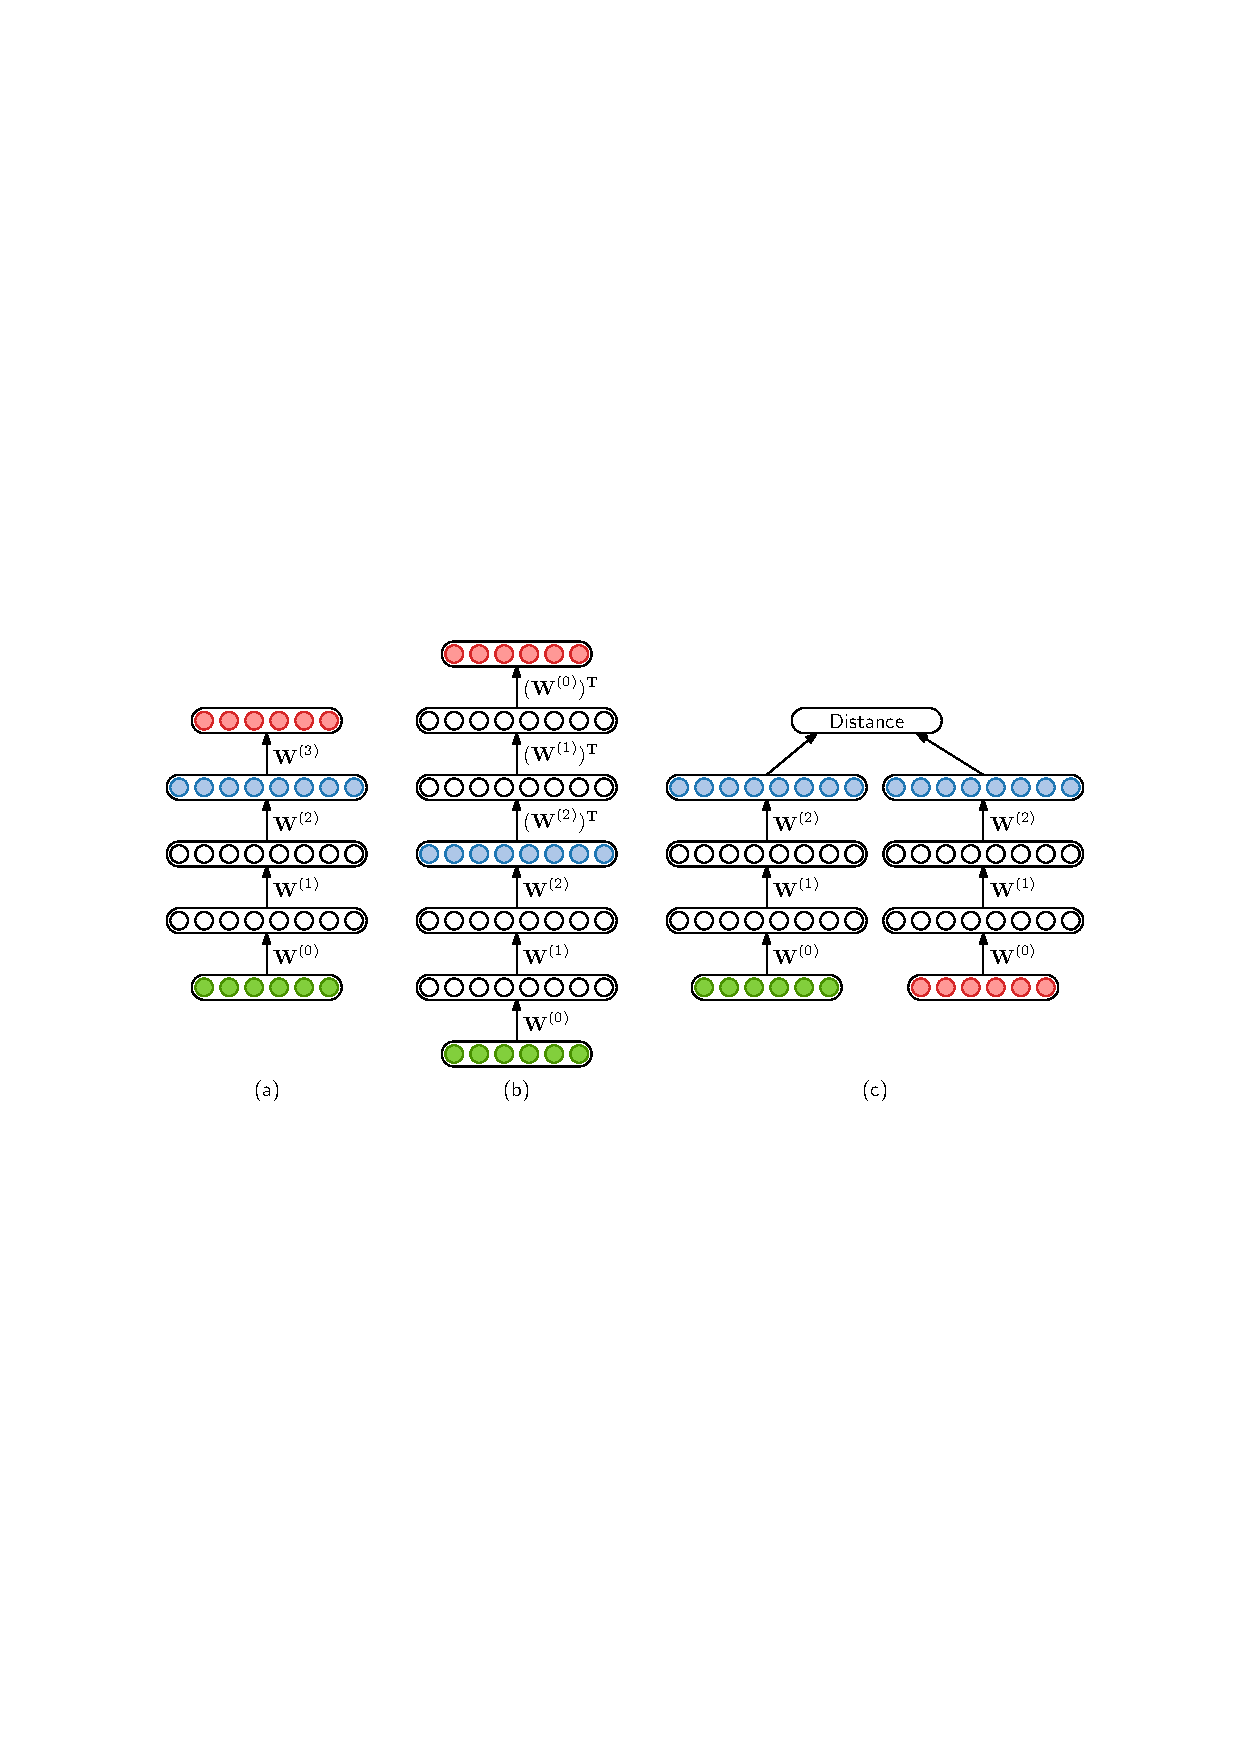
\includegraphics[width=\linewidth]{cae_siamese}
    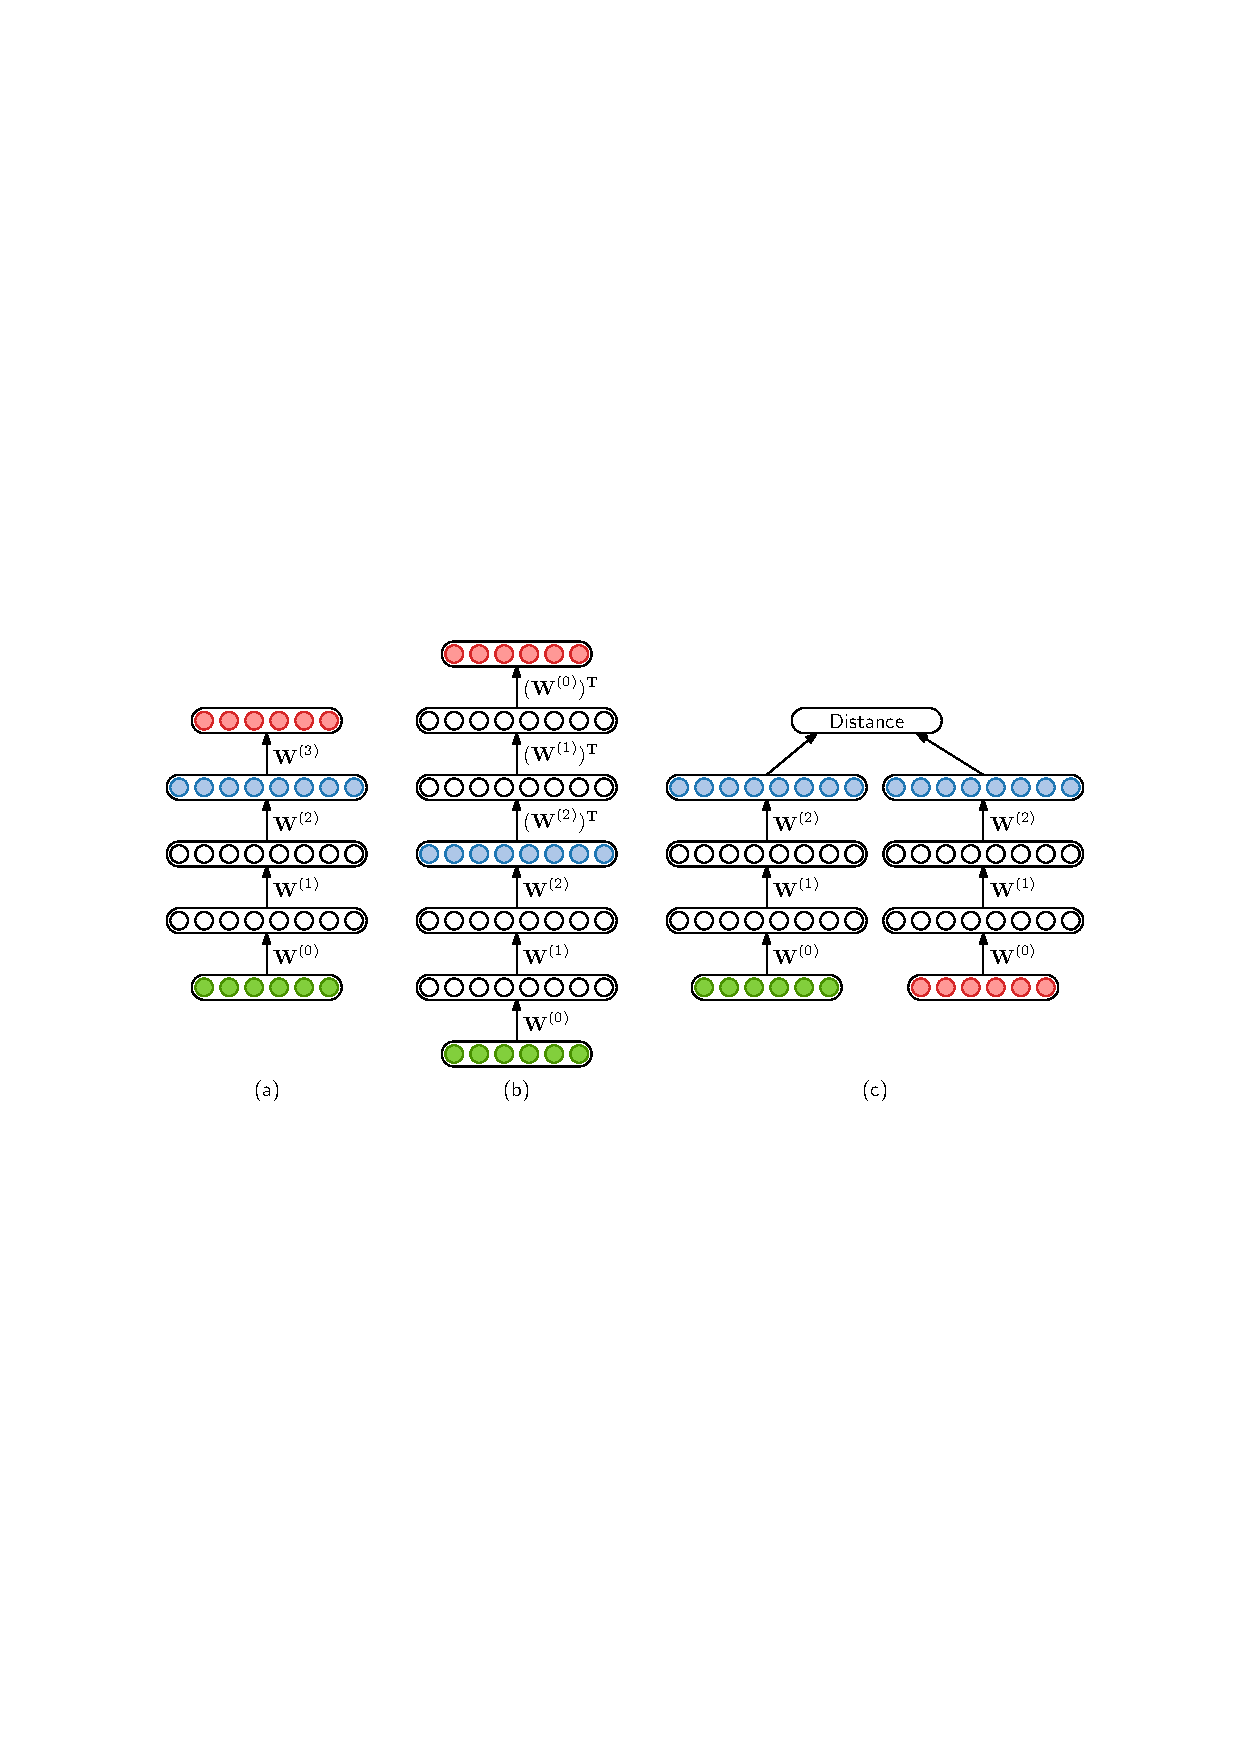
\includegraphics[width=0.918\linewidth]{cae_siamese}
    \caption[I am the short caption that appears in the list of figures, without references.]{
    (a) The cAE as used in this chapter. The encoding layer (blue) is chosen based on performance on a development set.
    (b) The cAE with symmetrical tied weights. The encoding from the middle layer (blue) is always used.
    (c) The siamese DNN. The cosine distance between aligned frames (green and red) is either minimized or maximized depending on whether the frames belong to the same (discovered) word or not.
    A cAE can be seen as a type of DNN~\cite{dahl+etal_taslp12}.
    }
    \label{fig:cae_siamese}
\end{figure}


The following is an example of an equation:
\begin{equation}
P(\vec{z} | \vec{\alpha}) = \int_{\vec{\pi}} P(\vec{z} | \vec{\pi}) \, p(\vec{\pi} | \vec{\alpha}) \, \textrm{d} \vec{\pi}
= \int_{\vec{\pi}} \prod_{k = 1}^K \pi_k^{N_k} \frac{1}{B(\vec{\alpha})} \prod_{k = 1}^K \pi_k^{\alpha_k - 1} \, \textrm{d} \vec{\pi}
\label{eq:example_equation}
\end{equation}
which you can subsequently refer to as~\eqref{eq:example_equation} or Equation~\ref{eq:example_equation}.
But make sure to consistently use the one or the other (and not mix the two ways of referring to equations).

\subsection*{Feature Extractors}


\subsubsection*{What is a feature Extractor}
A feature extractor is a computer vision algorithm or deep-learning model that identifies and extracts key features in an image. A feature is a pixel or weight of multiple pixels that represents a highly unique and distinctive part of an image. For instance, this could be an edge between a wall and the sky. Feature extractors are characterized by a spatial coordinate and a descriptor. A descriptor is a vector which contains information about the helps it be uniquely identified again in a new image. This can include information about the size, shape, and intensity of the feature. One can also infer the scale and orientation of the feature from the descriptor. A feature extractor also commonly includes a confidence score which indicates a score of how unique and well-defined the feature is. Ultimately, a feature extractors goal is to find unique and well-defined features that can be used to develop a complex understanding of the nuances and details of an image.
\subsubsection*{Usage in this task}
In this task, feature extractors are used to extract keypoints in images. These are used for intra-image rotational and translational estimates, and matching similar images. 



feature extractors are nb bc they r iinvariant to scale rotation and transformation. As opposed to simply correlating entire image. also less computationally expensive.
https://baotramduong.medium.com/feature-extraction-in-computer-vision-using-python-358d7c9863cb



common feature extraction techniques include edge detection, color histograms, and texture analysis



\section{Choosing a Feature Extractor}
When selecting a feature extractor, several critical factors must be considered:
\begin{itemize}
    \item \textbf{Accuracy:} The extractor needs to be accurate to ensure GPS inference is accurate. That is, the extractor should provide a sufficient quality and quantity of keypoints. This is quantified as subtending over 500 good matches from similar image pairs. 
    \item \textbf{Speed:} Be capable of real-time processing to ensure timely navigation and decision-making in dynamic environments. Specifically, initial tests must extract features in less than 1 second on a CPU. For the neural network-based models, the time taken to extract features must be less than 3 second on a CPU since they may be implemented with a GPU and CUDA libraries to improve performance. 
    \item \textbf{Robustness:} The feature extractor should exhibit invariance to changes in scale, rotation, illumination, perspective and noise to ensure accurate and repeatable performance across different flight datasets and conditions.
\end{itemize}

Feature extractors have different parameters trading-off accuracy and speed. For example, there are detection thresholds, descriptor sizes, and keypoint densities that can be adjusted to optimize performance. 

\section{Types of Feature Extractors}
\subsection{Traditional Feature Extractors}
\subsubsection{SIFT (Scale-Invariant Feature Transform)}
SIFT detects and describes local features in images. It is robust to changes in scale, rotation, and illumination, making it a reliable choice for many applications. However, its computational intensity can be a drawback in real-time scenarios.
\begin{itemize}
    \item \textbf{Advantages:} High accuracy and robustness due to its multi-scale approach and precise keypoint localization. SIFT's descriptors are highly distinctive, enabling reliable matching across different views and conditions.
    \item \textbf{Disadvantages:} High computational cost and slower processing speed due to the extensive keypoint detection and descriptor computation steps, making it less suitable for real-time applications.
\end{itemize}


\subsubsection{SURF (Speeded-Up Robust Features)}
SURF is a faster alternative to SIFT, utilizing integral images for rapid computation of image convolutions. It offers good accuracy and robustness while being computationally more efficient than SIFT.
\begin{itemize}
    \item \textbf{Advantages:} Faster than SIFT due to its use of Haar wavelets and integral images, providing good balance between speed and accuracy. It maintains robustness to scale and rotation changes.
    \item \textbf{Disadvantages:} Still relatively computationally expensive compared to simpler methods like ORB, and can be less accurate than SIFT in certain complex scenarios.
\end{itemize}



\subsubsection{ORB (Oriented FAST and Rotated BRIEF)}
ORB combines the FAST keypoint detector and the BRIEF descriptor, providing a highly efficient feature extraction method suitable for real-time applications. It is designed to be both fast and invariant to rotation and scale.
\begin{itemize}
    \item \textbf{Advantages:} High speed and efficiency, making it suitable for real-time applications. ORB's binary descriptors are computationally less intensive while providing sufficient discriminative power for many tasks.
    \item \textbf{Disadvantages:} Lower accuracy compared to SIFT and SURF, especially in complex scenes with significant variations in lighting and scale. The binary nature of BRIEF descriptors can sometimes lead to higher false match rates.
\end{itemize}

\subsection{AKAZE (Accelerated-Keypoint-Affine-Zernike)}
AKAZE is a feature extraction method that combines speed and accuracy by using nonlinear scale space and feature detection. It is designed to be robust to various transformations and lighting conditions.
\begin{itemize}
    \item \textbf{Advantages:} High speed and efficiency due to its nonlinear scale space and feature detection approach. AKAZE is robust to scale, rotation, and illumination changes, making it suitable for diverse environments.
    \item \textbf{Disadvantages:} May not be as accurate as SIFT or SURF in certain scenarios, particularly those with complex textures or repetitive patterns. The trade-off between speed and accuracy may vary depending on the application.
\end{itemize}

\subsection{Deep Learning-Based Feature Extractors}
Deep learning-based feature extractors leverage neural networks to learn feature representations directly from data. These models need to be trained on large datasets to capture complex and hierarchical features effectively. They offer high accuracy and the ability to adapt to specific tasks through transfer learning.
    \item \textbf{Advantages:} High accuracy and the ability to learn complex and hierarchical features directly from data, enabling robust performance across diverse tasks and conditions. 
    \item \textbf{Disadvantages:} Requires substantial computational resources for training and inference. The training process is data-intensive, requiring large labeled datasets to achieve optimal performance.
\end{itemize}

\subsubsection{Pre-trained Models (SuperPoint)}
Utilizing pre-trained models, like Superpoint, that are trained on large datasets are often highly accurate relative to their efficiency. They are trained on a variety of datasets and aim to generalize well to a variety of tasks.
\begin{itemize}
    \item \textbf{Advantages:} High accuracy due to extensive pre-training on large and diverse datasets. 
    \item \textbf{Disadvantages:} May not generalize well to specific datasets which are not representative of the application dataset.
\end{itemize}



\section{Evaluation for UAV-Based Navigation}
\subsection{Requirements}
For the Skripsie project, the feature extractor must meet the following initial requirements with default parameters:
\begin{itemize}
    \item 
    \item 
    \item Must be free to use and not require any pre-training or live-training. The former excludes SURF, SIFT, and the latter, deep learning-based models. 
\end{itemize}

\subsection{Recommended Feature Extractors}
The feature extractor should be applicable to application specific requirements. In the case of this project, it should be free to use and not require any pre-training or live-training due to scope. As such, the following feature extractors are recommended:
\begin{itemize}
    \item ORB: A fast and efficient feature extractor that provides a good balance between speed and accuracy. It is suitable for real-time applications and can handle scale and rotation changes effectively.
    \item AKAZE: A feature extraction method that combines speed and accuracy by using nonlinear scale space and feature detection. It is robust to various transformations and lighting conditions.
    \item SuperPoint: A pre-trained model that offers high accuracy and efficiency for real-time applications. It learns feature representations directly from data, making it adaptable to specific tasks.


    


\chapter{Results}

TESTS:
amt of keypoints for a specific runtime that are accepted as good matches
overall accuracy for heading and GPS change estimation


DATASET PARAMETERS:
image resolution vs speed accuracy
dataset terrain



All parameter choices




test 1: accuracy on a single dataset for rotational estimation (global matcher), global matching technique, and local matcher. gonna need to split those. say something about the matches are good no matter what  - not a hard task.
So test both methods (Plus neural local) on both stages (2x3 results) on a single dataset - see which is more accurate only. - total time and acc.
test 2: Take the top 3 combinations and test them on all the datasets (or as many as are close together in accuracy) - optimize for datasets - see which is more accurate only. - total time and acc. 
test 3: mess up the parameters and see how it affects the stability of different methods as well as the overall accuracy - stability, acc and time. 
test 4: test whether one performs significantly better than normally when used as the global matcher technique

XXX - note that we dont look at time per extraction as the time of latter stages is affected by the amount and quality of keypoints. So it might extract rubbish faster, but then take longer to match. So we look at total time.
Test 1 and 2 show accuracy. Test 2 and 3 show robustness. 

XXX - need to make a note on why mean heading error is not compared much - it subtends GPS error - and its estimated in this project as we dont have an accurate heading. 

XXX - say we are going to use histograms, its significantly faster, ensures no effects from the global match, could potentially test that after 







On face value, ORB has more accuracy and less time per keypoint extracted, and less total time in the most recent example. However, one also notes how the time varies significantly as the maximum number of keypoints increases. 

AKAZE has a filter threshold which is difficult to tune and highly sensitive to minor changes. Further, this threshold needs to be changed based on the dataset depending on the types of keypoints and visibility etc. As such, it is easier to use the more simple and consistent number of keypoints threshold that ORB uses. To summarize it, ORB is much easier to tune, and tends to have a higher accuracy to time ratio. To achieve the same top local minimum error, AKAZE subtends a runtime of 712 seconds, while ORB subtends a runtime of 271 seconds. This is a significant difference. 

However, AKAZE is significantly more accurate at the same time to run and time per keypoint extracted. It is also more robust to changes in the dataset. Further, a change in time does not subtend a large change in accuracy. However, AKAZE extracts much less, and higher quality keypoints. This is advantageous for efficiency and accuracy, however, it makes AKAZE highly volatile to varying datasets as it will often not acquire sufficient keypoints. This can be mitigated by having an adaptive good match filtering threshold (this is implemented). However, the AKAZE threshold still needs to be manually tuned, this can also be made dynamic, at a time cost for constant re-estimation. 

However, when trying different data sets etc - and perhaps when trying it with the local matcher, robustness might affect these end results. 





NOTE ORB simply does not work on the desert dataset 





Please note that these tests are run without optimal settings - i.e. for debug purposes certain parts run which normally would not. 




TEST 1:
Heading estimation error too high.
Heading estimation error too high.
Linear regression inferred factor x: 3.207310914993286
Linear regression inferred factor y: 3.526571035385132 

Heading estimation error too high.
Heading estimation error too high.
Heading estimation error too high.
Heading estimation error too high.
Stability analysis mean (relative to src - best result) and var*10e6
Phase Correlation stability: 1.159 +/- 68807.336
Linear Algebra stability: 1.000 +/- 56.929
Affine stability: 1.020 +/- 921.300
Rigid stability: 0.995 +/- 160.067
Homography stability: 1.108 +/- 5592.924

Percentage Deviation: [3.22100261] %
Preprocessing Global Detector: ORB, Preprocessing Global Matcher: BF, Global Matching Technique: Histogram, Local Detector: ORB, Local Matcher: BF
Mean normalized GPS error: [24.86177763]
 Mean Heading Error: 1.9734131972502695
Mean Length of Global Keypoints: 5426.8
Mean Length of Local Keypoints: 5426.8
Mean Global Time to Extract Keypoints: 0.0295 s
Mean Number of Good Matches: 604.5387931034483
Range of Good Matches: 7310
Time taken to execute The Method: 57.5468 seconds



END 1

Heading estimation error too high.
Heading estimation error too high.
Linear regression inferred factor x: 3.2284045219421387
Linear regression inferred factor y: 3.480206251144409

Heading estimation error too high.
Heading estimation error too high.
Heading estimation error too high.
Heading estimation error too high.
Stability analysis mean (relative to src - best result) and var*10e6
Phase Correlation stability: 1.163 +/- 68807.336
Linear Algebra stability: 1.000 +/- 43.544
Affine stability: 1.026 +/- 595.532
Rigid stability: 0.994 +/- 195.841
Homography stability: 1.111 +/- 5592.908

Percentage Deviation: [3.11905048] %
Preprocessing Global Detector: ORB, Preprocessing Global Matcher: BF, Global Matching Technique: Histogram, Local Detector: AKAZE, Local Matcher: BF
Mean normalized GPS error: [24.07484528]
 Mean Heading Error: 1.9734131972502695
Mean Length of Global Keypoints: 5426.8
Mean Length of Local Keypoints: 9987.666666666666
Mean Global Time to Extract Keypoints: 0.0337 s
Mean Number of Good Matches: 604.5387931034483
Range of Good Matches: 7310
Time taken to execute The Method: 67.8058 seconds


END 2

Stability analysis mean (relative to src - best result) and var*10e6
Phase Correlation stability: 1.190 +/- 68807.336
Linear Algebra stability: 1.000 +/- 176.334
Affine stability: 1.101 +/- 2279.378
Rigid stability: 0.989 +/- 473.279
Homography stability: 1.141 +/- 5715.823

Percentage Deviation: [2.75680053] %
Preprocessing Global Detector: ORB, Preprocessing Global Matcher: BF, Global Matching Technique: Histogram, Local Detector: SUPERPOINT, Local Matcher: LightGlue
Mean normalized GPS error: [21.27876627]
 Mean Heading Error: 1.9734131972502695
Type: Numpy Array
Shape: torch.Size([1, 1000, 2])
Mean Length of Global Keypoints: 5426.8
Mean Length of Local Keypoints: 1000.0
Range of Local kp: 0
Mean Global Time to Extract Keypoints: 0.0342 s
Mean Number of Glob good Matches: 604.5387931034483
Time taken to execute The Method: 130.9345 seconds

Note that superpoint and Lightglue have various tunable parameters. However, there is no way to reduce the time taken to extract and match keypoints to the point of the algorithmic models without significantly reducing accuracy. However, these models are significantly faster on GPU's and CUDA libraries. There is a decent range where one can increase time cost and gain a reasonable increase in accuracy. Superpoint and LightGLue parameters are relatively hard to tune, as there are many. However, XXX, its yet to be seen how robust these parameters are to different datasets. 

END 3


Heading estimation error too high.
Stability analysis mean (relative to src - best result) and var*10e6
Phase Correlation stability: 0.877 +/- 70819.259
Linear Algebra stability: 1.000 +/- 62.694
Affine stability: 0.998 +/- 1355.790
Rigid stability: 0.987 +/- 181.514
Homography stability: 1.044 +/- 6260.942

Percentage Deviation: [3.05771815] %
Preprocessing Global Detector: AKAZE, Preprocessing Global Matcher: BF, Global Matching Technique: Histogram, Local Detector: ORB, Local Matcher: BF
Mean normalized GPS error: [20.64342049]
 Mean Heading Error: 1.7089258086216432
Mean Length of Global Keypoints: 55.53333333333333
Mean Length of Local Keypoints: 5426.8
Range of Local kp: 7310
Mean Global Time to Extract Keypoints: 0.2273 s
Mean Number of Glob good Matches: 300.0
Time taken to execute The Method: 26.1905 seconds


END 4


Stability analysis mean (relative to src - best result) and var*10e6
Phase Correlation stability: 0.905 +/- 70819.259
Linear Algebra stability: 1.000 +/- 166.490
Affine stability: 1.044 +/- 2069.720
Rigid stability: 0.983 +/- 324.556
Homography stability: 1.077 +/- 6339.018

Percentage Deviation: [2.77759658] %
Preprocessing Global Detector: AKAZE, Preprocessing Global Matcher: BF, Global Matching Technique: Histogram, Local Detector: SUPERPOINT, Local Matcher: LightGlue
Mean normalized GPS error: [18.75224969]
 Mean Heading Error: 1.7089258086216432
Mean Length of Global Keypoints: 55.53333333333333
Mean Length of Local Keypoints: 1000.0
Range of Local kp: 0
Mean Global Time to Extract Keypoints: 0.2408 s
Mean Number of Glob good Matches: 300.0
Time taken to execute The Method: 77.1795 seconds

END 5








Another note, this data is run in debug mode, with many methods running sequentially instead of a single method. Further, this is ran in a high accuracy mode for both, with an aim to get good results for both while keeping the time between methods reasonably similar without moving far off optimal points. 








ADDITIONAL TEST:
Percentage Deviation: [2.65627788] %
Preprocessing Global Detector: AKAZE, Preprocessing Global Matcher: BF, Global Matching Technique: Histogram, Local Detector: AKAZE, Local Matcher: BF
Mean normalized GPS error: [18.24802137]
 Mean Heading Error: 1.545597672500035
Mean Length of Global Keypoints: 4083.133333333333
Mean Length of Local Keypoints: 15055.266666666666
Range of Local kp: 12695
Mean Global Time to Extract Keypoints: 0.2440 s
Mean Number of Glob good Matches: 300.0
Time taken to execute The Method: 113.2767 seconds
with akaze 0.00017, and 0.00007 for local. 



akaze akaze:
Phase Correlation stability: 0.902 +/- 46811.385
Linear Algebra stability: 1.000 +/- 38.748
Affine stability: 1.023 +/- 805.875
Rigid stability: 0.986 +/- 202.970
Homography stability: 1.114 +/- 5841.347

Percentage Deviation: [2.80564334] %
Preprocessing Global Detector: AKAZE, Preprocessing Global Matcher: BF, Global Matching Technique: Histogram, Local Detector: AKAZE, Local Matcher: BF
Mean normalized GPS error: [19.27412787]
 Mean Heading Error: 1.6004082453122863
Mean Length of Global Keypoints: 1296.9333333333334
Mean Length of Local Keypoints: 15055.266666666666
Range of Local kp: 12695
Mean Global Time to Extract Keypoints: 0.2092 s
Mean Number of Glob good Matches: 300.0
Time taken to execute The Method: 56.3528 seconds


akaze orb (local):
XXX make note abt dynamic adjustment 

The next critical feature in an image-based navigation system is the feature matcher. The feature matcher serves two main purposes. The first is to find the most highly correlated image pair. The second is to estimate the relative pose (translation and rotation) between the two images. Thus, we break up this section into two components, global matching and local matching. 
xxx check scale if or not if
To compute matches, The descriptor first transforms each feature individually to a normalized space. This process aligns the feature’s orientation, adjusts scale, and normalizes other factors like intensity, ensuring that each descriptor is in a consistent format for direct comparison during matching.


Matches have specific confidence levels. When calculating transformations we can include confidence weightings to improve the accuracy of the estimations. 

Broadly speaking there are two types of feature matchers: local and global. Local matchers are used to find the relative pose between two images. Global matchers are used to find the correlation between two images.

\section*{Local Matchers}
\subsection*{Brute-Force Matcher (BFMatcher)} BFMatcher compares every descriptor from one image with all descriptors in another image to find the closest match. It calculates the distance between descriptors using a chosen metric (e.g., Euclidean for SIFT, Hamming for ORB). Matches are sorted by distance, and the best ones are selected. While simple and effective, it can be slow with large datasets. Best suited for smaller datasets or when precision is prioritized over speed.

\subsection*{FLANN (Fast Library for Approximate Nearest Neighbors)} FLANN is an efficient matcher that uses approximate nearest neighbor search, speeding up the matching process, especially for large datasets. It uses tree-based algorithms or k-means clustering to quickly find matches. FLANN is often preferred for tasks involving large datasets where speed is critical, such as real-time applications with SIFT or SURF descriptors. FLANN must be used with Local-sensitivity hashing to allow for operations on its binary descriptors. 



\subsection*{Light Glue} Light Glue is a lightweight, relative to other neural network approaches, neural network-based matcher that uses deep learning to match features across images. It is optimized for speed and memory efficiency, making it suitable for mobile and embedded systems. Light Glue provides robust matches even under challenging conditions, such as significant viewpoint changes or lighting variations. This is a significant improvement over traditional feature matching methods like BF or FLANN matchers, however, it increases computational time and risks an inability to generalize well, especially in this context which is unlikely to have training data based off UAV images.

\section*{Improvements to Matching techniques}
\subsection*{Cross-Check Matching} Cross-check matching performs matching in both directions (from image A to B and B to A) and only retains matches that are consistent in both directions. This reduces false positives and increases the reliability of matches. However, this doubles the computation time.
 

\subsection*{RANSAC (Random Sample Consensus)} RANSAC is used to refine matches by identifying and removing outliers. It works by iteratively selecting a subset of matches, estimating a model (e.g., homography), and checking how well the remaining matches fit this model. Matches that deviate significantly are considered outliers and discarded. RANSAC is crucial in tasks like image stitching, where accurate geometric transformations are required.


\subsection*{SuperGlue} SuperGlue is a more advanced neural network-based matcher that leverages attention mechanisms, dynamically aggregating local features based on their inferred importance, to enhance the matching process. It works by learning to match keypoints directly from image data, providing superior performance in complex scenarios with large changes in scale, rotation, or perspective. SuperGlue is well-suited for high-precision applications like 3D reconstruction. 


\section*{Global Matchers}

Global matchers aim to capture the overall similarity between images. Many techniques, like local matchers, do not inherently test similarity evenly across the image and therefore may tend to compare local zones instead of the entire context. This leads to sub-par matching and pose inference. 
To ensure full context, we can either choose a global matcher that already considers the entire image space, or use one that does not and divide into grids and compare per-grid to ensure complete context. In both cases, the scale and rotation should be normalized between images unless explicitly invariant to these. 
The following are chosen based on their ability to be computationally efficient and not require any pre- or live-training.

\subsection*{Translation affects the results of these}

\subsection*{Local matching conversion techniques}
These are techniques which convert local matchers, which are translation invariant, into techniques which penalize translation in its score. From the above local matchers, tests will be conducted on 

\subsection*{Histograms}

\subsection*{Hashing Methods}  
Hashing methods, like LSH (Local-sensitivity hashing) or PCA (Principal-component analysis), map high-dimensional descriptors to a lower-dimensional space. Hashing focuses on descriptor similarity rather than relative spatial positions within the image. Grid-rot apply

\subsection*{SSIM (Structural Similarity Index)}  
SSIM compares images based on luminance, contrast, and structural information, making it sensitive to spatial shifts like translation. 

\subsection*{KNN or other local Matching}  
Adapting local matchers, such as AKAZE, for global matching allows for high accuracy. 

Use low threshold, per-grid matching, and count the amount of matches. This is point-to-point and can be computationally expensive when comparing many images. 



\subsubsection*{Plan}
These methods offer complex tradeoffs within different accuracy and speed metrics. As such, tests will be conducted on individual methods as well as hybrid approaches. All of the above methods will be included in these tests except the deep-learning approaches which are too computationally intensive for the task of finding the most correlated image. The best method is that which results in the combination of image pairs (matches) which subtends the lowest mean squared deviation in actual and estimated GPS locations and heading. 


To summarize: the invariant methods are: Hashing, BOVW; variant methods are 



Intermediary results:

These results indicate the time to complete the set of best correlated images. The score has not been used as the highly variant parameter set often, with enough computation, can achieve the correct score. So instead of holding computational time constant, which is not clear, we increase the parameters until we see it achieve the correct score. Then the time is recorded and a higher accuracy is dually implied in a lower time. Where excessive time is required and the correct combination has not been met, there will be an indication of failure to meet score. 
Excessive time is defined as greater than 10s for an image space of 12. 

\begin{table}[H]
    \centering
    \begin{tabular}{|c|c|}
    \hline
    \textbf{Search Space (Images)} & \textbf{Runtime (Seconds)} \\ \hline
    12  & 5.04 \\ \hline
    11  & 5.14 \\ \hline
    10  & 4.90 \\ \hline
    9   & 4.30 \\ \hline
    8   & 3.74 \\ \hline
    7   & 3.56 \\ \hline
    6   & 3.12 \\ \hline
    5   & 2.59 \\ \hline
    4   & 1.99 \\ \hline
    3   & 1.51 \\ \hline
    2   & 0.98 \\ \hline
    1   & 0.49 \\ \hline
    \end{tabular}
    \caption{KNN Matching: Search Space vs. Runtime}
    \end{table}

For BF_matching with KNN search, the run-time per image is roughly half a second, and the time complexity is linear.   

\section*{Concept}

The flow of the camera system shall be as follows:

\begin{enumerate}
    \item The controller shall receive footage in real-time from the UAV and sync it with known telemetry data such as GPS coordinates, altitude, heading and speed.
    \item The controller shall then process the video footage and telemetry data to extract and store the relevant features
    \item When the GPS signal is lost, the UAV will turn around
    \item The controller shall extract and match the features of the current image with that of the previous images
    \item It will find the most correlated images and use that image to determine the change in feature locations to infer the UAV's position
\end{enumerate}




XXX - flat earth buildings assumption
XXX - try 512 x 512
XXX - different datasets


\section{Rotational Estimators}

\subsection{Introduction}
Rotational estimators are critical in image alignment and pose estimation tasks. In this project, rotational estimators are employed to align UAV-captured images when GPS data is unreliable. The accuracy of rotational alignment directly impacts the estimation of translational shifts and image similarity. These steps are crucial to ensuring reliable navigation in GPS-denied environments.

Four methods were selected for rotational estimation based on their applicability, computational efficiency, and accuracy. Other methods were considered but ultimately excluded due to their efficiency or accuracy.   

\subsection{Methods}
\begin{itemize}
    \item \textbf{Homography Estimation}: A method supporting 8 degrees of freedom (DoF), accounting for rotation, scaling, translation, and perspective correction. It is suitable for complex transformations but may introduce unnecessary errors when perspective correction is not needed.
    \item \textbf{Affine Estimation}: A method with 6 degrees of freedom that handles rotation, scaling, and translation without perspective correction. It is computationally efficient and offers sufficient transformation handling for most tasks.
    \item \textbf{2x2 Rotation Matrix}: A simplified method that accounts only for rotational and translational freedom. It lacks support for scaling and perspective, making it less effective for complex transformations.
    \item \textbf{Vector-based Estimation}: A direct estimation of rotation using vectors derived from image points. This method lacks robust outlier removal and complexity, limiting its effectiveness for real-world applications.
\end{itemize}

\textbf{Conclusion:} These methods were chosen to provide a range of complexity and computational efficiency, with homography and affine estimation being the primary focus due to their broader applicability in image transformations.

\subsection{Improvement Techniques}
To enhance the accuracy and robustness of these methods, the following improvement techniques were applied:
\begin{itemize}
    \item \textbf{Lowe's Ratio with KNN}: Filters out ambiguous matches by comparing the best match with the second-best match, effectively eliminating outliers, especially in repetitive or noisy data.
    \item \textbf{RANSAC (Random Sample Consensus)}: A robust outlier removal technique that iteratively refines the inlier set to accurately estimate transformations.
    \item \textbf{Confidence Thresholds}: Filters out matches or keypoints below a certain confidence level. In practice, this technique performed worse than Lowe's Ratio and RANSAC, and when used alongside them, it reduced accuracy due to over-filtering.
    \item \textbf{Confidence Weightings}: Adjusts the influence of each match based on its confidence score. Similar to confidence thresholds, this technique led to decreased stability by over-filtering.
\end{itemize}

\textbf{Conclusion:} The combination of Lowe's Ratio and RANSAC was the most effective in improving accuracy and robustness. Confidence thresholds and weightings were found to be redundant.

\subsection{Initial Accuracy Testing}
Initial tests were conducted using relatively optimal parameters, and the performance of each method was evaluated based on its Mean Absolute Error (MAE) in heading relative to the ground truth. The results are summarized below:

\begin{table}[H]
    \centering
    \begin{tabular}{|c|c|c|}
        \hline
        \textbf{Method} & \textbf{MAE (heading)} & \textbf{Result} \\
        \hline
        Homography & 0.1207 & Accurate \\  
        Affine & 0.1129 & Best-performing \\  
        2x2 Rotation Matrix & 1.0277 & Poor performance \\  
        Vector-based & 7.3571 & Poor performance \\  
        \hline
    \end{tabular}
    \caption{Initial Testing Results (MAE - Mean Absolute GPS Error)}
\end{table}

\textbf{Conclusion:} The affine method achieved the lowest MAE, making it the most accurate for aligning images. Homography performed slightly worse due to its additional degrees of freedom, which introduced unnecessary errors. The 2x2 rotation matrix and vector-based methods were unsuitable for the task due to their lack of transformation handling complexity. Based on these results, affine and homography were selected for further testing.

\subsection{Accuracy in Global and Local Matching}
To assess the overall suitability of the rotational estimators, it is crucial to evaluate their impact on the system as a whole. Focusing solely on heading errors does not capture the full extent of how minor inaccuracies propagate through the system. By examining the Mean Normalized Error (MNE) in GPS coordinates, a more realistic understanding of the cumulative effect of small rotational errors and their influence on overall system performance is obtained.

\begin{table}[H]
    \centering
    \begin{tabular}{|c|c|c|}
        \hline
        \textbf{Global Method} & \textbf{Local Method} & \textbf{Mean Normalized Error (GPS)} \\  
        \hline
        Homography & Homography & 48.90 \\  
        Homography & Affine & 41.80 \\  
        Affine & Homography & 42.37 \\  
        Affine & Affine & 41.28 \\  
        \hline
    \end{tabular}
    \caption{Accuracy Comparison for Global and Local Matching Techniques (MNE - Mean Normalized Error)}
\end{table}

\textbf{Conclusion:} The affine method consistently outperforms homography in both global and local matching scenarios. The significant reductions in GPS error, even with relatively minor decreases in rotational error, highlight the sensitivity of both methods to rotational inaccuracies. This underscores the critical importance of optimizing the accuracy of the rotational stage.


\subsection{Time Constraints}
Time efficiency was evaluated to assess the computational performance of each method. The table below summarizes the average, minimum, median, and maximum runtimes for each approach. Lower computation times enable higher frame rates, provide greater tolerance for minor errors, and allow for faster processing of larger search spaces, ultimately improving accuracy.


\begin{table}[H]
    \centering
    \begin{tabular}{|c|c|c|c|c|}
        \hline
        \textbf{Method} & \makecell{\textbf{Mean Time} \\ \textbf{(ms)}} & \makecell{\textbf{Max Time} \\ \textbf{(ms)}} & \makecell{\textbf{Min Time} \\ \textbf{(ms)}} & \makecell{\textbf{Median Time} \\ \textbf{(ms)}} \\
        \hline
        Affine & 1.276 & 11.55 & 0.00 & 0.999 \\  
        Homography & 22.58 & 50.74 & 0.98 & 10.80 \\  
        \hline
    \end{tabular}
    \caption{Time Analysis for Affine and Homography Methods}
\end{table}

\textbf{Conclusion:} Affine is significantly faster than homography, with a much lower mean and median runtime. The greater variability in homography’s runtime (indicated by the difference between mean and median) is due to its handling of more complex transformations. Affine’s speed makes it particularly well-suited for real-time UAV applications.

\subsection{Robustness Testing}
Robustness testing was performed to assess each method's sensitivity to different parameter settings, such as RANSAC thresholds, Lowe’s ratio for match filtering, and keypoint confidence thresholds. These tests are essential to determine the methods’ reliability under varying conditions and data quality.

\subsubsection{RANSAC Threshold Testing}
We varied RANSAC thresholds to evaluate how sensitive each method is to outlier removal. A lower threshold implies more aggressive filtering, which reduces the number of keypoints but increases the reliability of those retained.

\begin{table}[H]
    \centering
    \begin{tabular}{|c|c|c|}
        \hline
        \textbf{Threshold} & \makecell{\textbf{Homography (Mean} \\ \textbf{Heading Error)}} & \makecell{\textbf{Affine (Mean} \\ \textbf{Heading Error)}} \\
        \hline
        0.2 & 0.1384 & 0.1089 \\  
        0.5 (Default) & 0.1207 & 0.1129 \\  
        5 & 0.1249 & 0.1003 \\  
        25 & 0.1222 & 0.0997 \\  
        50 & 0.1226 & 0.1112 \\  
        \hline
    \end{tabular}
    \caption{Effect of RANSAC Thresholds on Heading Error}
\end{table}

\textbf{Conclusion:} Both methods are robust to RANSAC threshold changes, but homography exhibits greater variability at lower thresholds, suggesting a weaker estimation capability when fewer keypoints are available.

\subsubsection{Lowe's Ratio Testing}
We evaluated Lowe's ratio to assess its impact on match filtering and rotational estimation accuracy. A lower ratio implies more aggressive filtering, reducing the number of matches but increasing their quality.

\begin{table}[H]
    \centering
    \begin{tabular}{|c|c|c|}
        \hline
        \textbf{Lowe's Ratio} & \makecell{\textbf{Homography (Mean} \\ \textbf{Heading Error)}} & \makecell{\textbf{Affine (Mean} \\ \textbf{Heading Error)}} \\
        \hline
        0.6 & 0.1289 & 0.1098 \\  
        0.7 & 0.1255 & 0.1006 \\  
        0.8 & 0.1207 & 0.0997 \\  
        0.9 & 0.1139 & 0.1111 \\  
        0.95 & 0.1211 & 0.1054 \\  
        \hline
    \end{tabular}
    \caption{Effect of Lowe's Ratio on Heading Error}
\end{table}

\textbf{Conclusion:} Both methods are robust to changes in Lowe’s ratio. 

\subsubsection{Keypoint Confidence Threshold Testing}
Keypoint confidence thresholds were varied to evaluate how each method performs with different levels of keypoint quality. Lower thresholds admit more keypoints but decrease the reliability of individual keypoints.

\begin{table}[H]
    \centering
    \begin{tabular}{|c|c|c|}
        \hline
        \makecell{\textbf{Keypoint Confidence} \\ \textbf{Threshold}} & \makecell{\textbf{Homography (Mean} \\ \textbf{Heading Error)}} & \makecell{\textbf{Affine (Mean} \\ \textbf{Heading Error)}}\\
        \hline
        0.001 & 0.1404 & 0.1019 \\  
        0.0008 & 0.1207 & 0.0974 \\  
        0.0005 & 0.1247 & 0.0997 \\  
        0.0002 & 0.1247 & 0.1024 \\  
        \hline
    \end{tabular}
    \caption{Effect of Keypoint Confidence Thresholds on Heading Error}
\end{table}

\textbf{Conclusion:} Both methods are robust to changes in keypoint confidence thresholds, but affine remains more consistent at lower thresholds, maintaining lower mean errors with noisier keypoints.

\subsubsection{Overall Robustness}
In summary, affine consistently outperforms homography in terms of robustness, particularly in scenarios involving noisier or fewer keypoints. This makes affine the preferred method for handling datasets with varying quality and practical applications requiring stability under changing conditions.

\subsection{Conclusion}
Affine estimation is selected as the primary method for future work due to its superior accuracy, faster computation, and greater robustness. Its 6 degrees of freedom provide sufficient understanding of image transformations without introducing unnecessary errors from perspective correction. 


Best Rotator: Affine, AKAZE AND BF




\subsection*{Matching filtration techniques}
Global point matching. In order to find an accurate rotational estimate, we need to ensure that the points we use in the inference are of sufficient quality and quantity. This involves filtering out lower quality keypoints while considering sufficient keypoints are still needed to remove noise from resolution and computation limits and distortion-based point differences. This means we need to filter the matches between images. The first is to remove ambiguous matches. This involves using Lowes Ratio's Test to ensure the two best potential matches are sufficiently different based on their descriptors. Then, we can sort the matches according to how close the match is to its actual corresponding keypoint based on their descriptors. Finally, we can use homography and RANSAC to firstly estimate a model for the data points and reject any outliers to this model. Together, these steps remove ambiguity, ensure matches are of high quality, and remove outliers to ensure the best possible rotational estimate.
The three parameters associated with each of these steps are:
\begin{itemize}
    \item \textbf{Lowes Ratio Test}: This is the ratio of the distance of the best match to the second-best match. If this ratio is above a certain similarity allowed threshold, the match is considered ambiguous and removed. 
    \item \textbf{Homography and RANSAC}: The homography and RANSAC model is used to estimate the transformation between the two images. The RANSAC threshold is the maximum distance a point can be from the model to be considered an inlier. 
    \item \textbf{Keypoint Confidence Threshold}: This is the minimum confidence a keypoint must have to be considered in the matching process. This may be only keeping some number of the highest quality keypoints or keeping all keypoints above a certain similarity threshold. The former will be used as this ensures that we do not have to constantly adjust the threshold based on the dataset and quality, instead we are guaranteed to have a certain number of keypoints which is more important than being pedantic about the quality of the keypoints.
\end{itemize}
    
Note, this is tested on only the global matcher, and with multimethod, implying isolation in its effect on the rotational estimation. XXX this still now needs to be tested with the global matcher being the local matcher (added inferred effect) and on the local matcher. 
    Testing Kp threshold confidences:



    
AKAZE NO FILTER:
Percentage Deviation: [4.91698283] %
Preprocessing Global Detector: AKAZE, Preprocessing Global Matcher: BF, Global Matching Technique: Histogram, Local Detector: AKAZE, Local Matcher: BF
Mean normalized GPS error: [65.07094916]
 Mean Heading Error: 0.8556339319426911
Mean Length of Keypoints: 2525.866666666667
Mean Global Time to Extract Keypoints: 0.2709 s
Mean Number of Good Matches: 802.4396551724138
Range of Good Matches: 1524
Time taken to execute The Method: 45.7884 seconds

AKAZE 500
Percentage Deviation: [4.58746506] %
Preprocessing Global Detector: AKAZE, Preprocessing Global Matcher: BF, Global Matching Technique: Histogram, Local Detector: AKAZE, Local Matcher: BF
Mean normalized GPS error: [62.34674896]
 Mean Heading Error: 0.9235667588307905
Mean Length of Keypoints: 2525.866666666667
Mean Global Time to Extract Keypoints: 0.4008 s
Mean Number of Good Matches: 500.0
Range of Good Matches: 1524
Time taken to execute The Method: 62.8682 seconds



AKAZZE 300
Percentage Deviation: [4.53573965] %
Preprocessing Global Detector: AKAZE, Preprocessing Global Matcher: BF, Global Matching Technique: Histogram, Local Detector: AKAZE, Local Matcher: BF
Mean normalized GPS error: [61.64376568]
 Mean Heading Error: 0.9238056255750251
Mean Length of Keypoints: 2525.866666666667
Mean Global Time to Extract Keypoints: 0.2578 s
Mean Number of Good Matches: 300.0
Range of Good Matches: 1524
Time taken to execute The Method: 45.2109 seconds



\begin{table}[H]
    \centering
    \begin{tabular}{|c|c|c|c|c|c|c|}
        \hline
        \makecell{\textbf{Keypoints} \\ \textbf{Allowed}} & \textbf{No Filter} & \textbf{500} & \textbf{300} & \textbf{No Filter} & \textbf{500} & \textbf{300} \\ 
        \hline
        \multicolumn{1}{|c|}{\textbf{Method}} & \multicolumn{3}{c|}{\textbf{AKAZE}} & \multicolumn{3}{c|}{\textbf{ORB}} \\
        \hline
        \makecell{\textbf{GPS Error}} & 65.07 & 62.35 & 61.64 & 54.10 & 56.72 & 60.64 \\  
        \hline
        \makecell{\textbf{Mean Number} \\ \textbf{of Good Matches}} & 802.44 & 500.0 & 300.0 & 718.15 & 500.0 & 300.0 \\  
        \hline
        \makecell{\textbf{Range of} \\ \textbf{Good Matches}} & 1524 & 1524 & 1524 & 0 & 0 & 0 \\  
        \hline
        \makecell{\textbf{Mean Length} \\ \textbf{of Keypoints}} & 2525.87 & 2525.87 & 2525.87 & 3000.0 & 3000.0 & 3000.0 \\  
        \hline
        \makecell{\textbf{Time Per Keypoint} \\ \textbf{Extraction (s)}} & 0.2709 & 0.4008 & 0.2578 & 0.0636 & 0.0916 & 0.0571 \\  
        \hline
        \makecell{\textbf{Time Taken} \\ \textbf{(seconds)}} & 45.79 & 62.87 & 45.21 & 48.08 &  47.3382 & 46.04 \\  
        \hline
    \end{tabular}
    \caption{Comparison of AKAZE and ORB Feature Matching Performance}
\end{table}




From this table, its clear the optimal point for ORB is without filtering the matches given that ORB was running with only 3000 keypoints. For AKAZE, this point is at 300. This optimal point is based mainly on accuracy with consideration for no large time difference. As visible, ORB outperforms AKAZE in accuracy given roughly similar time constraints. 


As visible, ORB outperforms AKAZE in accuracy given roughly similar time constraints. The time is also more consistent accross different datasets implying more robustness. 
\graphicspath{{conclusion/fig/}}

\chapter{Summary and Conclusion}
\label{chap:conclusion}

% Bibliography
\bibliography{mybib}

% End matter
\appendix
\chapter{Project Planning Schedule}
\makeatletter\@mkboth{}{Appendix}\makeatother
\label{appen:derivations_bigramseg}

This is an appendix.

\chapter{Outcomes Compliance}
\makeatletter\@mkboth{}{Appendix}\makeatother
\label{appen:derivations_bigramseg}

This is another appendix.

\end{document}

